\documentclass{article}
\iffalse
This file is protected by Copyright. Please refer to the COPYRIGHT file
distributed with this source distribution.

This file is part of OpenCPI <http://www.opencpi.org>

OpenCPI is free software: you can redistribute it and/or modify it under the
terms of the GNU Lesser General Public License as published by the Free Software
Foundation, either version 3 of the License, or (at your option) any later
version.

OpenCPI is distributed in the hope that it will be useful, but WITHOUT ANY
WARRANTY; without even the implied warranty of MERCHANTABILITY or FITNESS FOR A
PARTICULAR PURPOSE. See the GNU Lesser General Public License for more details.

You should have received a copy of the GNU Lesser General Public License along
with this program. If not, see <http://www.gnu.org/licenses/>.
\fi

\author{} % Force author to be blank
%----------------------------------------------------------------------------------------
% Paper size, orientation and margins
%----------------------------------------------------------------------------------------
\usepackage{geometry}
\geometry{
	letterpaper,			% paper type
	portrait,				% text direction
	left=.75in,				% left margin
	top=.75in,				% top margin
	right=.75in,			% right margin
	bottom=.75in			% bottom margin
 }
%----------------------------------------------------------------------------------------
% Header/Footer
%----------------------------------------------------------------------------------------
\usepackage{fancyhdr} \pagestyle{fancy} % required for fancy headers
\renewcommand{\headrulewidth}{0.5pt}
\renewcommand{\footrulewidth}{0.5pt}
\newcommand{\terminaloutput}[1]{\texttt{#1}}
\rhead{\small{Project ANGRYVIPER}}
%----------------------------------------------------------------------------------------
% Appendix packages
%----------------------------------------------------------------------------------------
\usepackage[toc,page]{appendix}
%----------------------------------------------------------------------------------------
% Defined Commands & Renamed Commands
%----------------------------------------------------------------------------------------
\renewcommand{\contentsname}{Table of Contents}
\renewcommand{\listfigurename}{List of Figures}
\renewcommand{\listtablename}{List of Tables}
\newcommand{\todo}[1]{\textcolor{red}{TODO: #1}\PackageWarning{TODO:}{#1}} % To do notes
\newcommand{\code}[1]{\texttt{#1}} % For inline code snippet or command line
%----------------------------------------------------------------------------------------
% Various pacakges
%----------------------------------------------------------------------------------------
\usepackage{hyperref} % for linking urls and lists
\usepackage{graphicx} % for including pictures by file
\usepackage{listings} % for coding language styles
\usepackage{rotating} % for sideways table
\usepackage{pifont}   % for sideways table
\usepackage{pdflscape} % for landscape view
%----------------------------------------------------------------------------------------
% Table packages
%----------------------------------------------------------------------------------------
\usepackage{tabularx} % c=center,l=left,r=right,X=fill
\usepackage{float}
\floatstyle{plaintop}
\usepackage[tableposition=top]{caption}
\newcolumntype{P}[1]{>{\centering\arraybackslash}p{#1}}
\newcolumntype{M}[1]{>{\centering\arraybackslash}m{#1}}
%----------------------------------------------------------------------------------------
% Block Diagram / FSM Drawings
%----------------------------------------------------------------------------------------
\usepackage{tikz}
\usetikzlibrary{shapes,arrows,fit,positioning}
\usetikzlibrary{automata} % used for the fsm
%----------------------------------------------------------------------------------------
% Colors Used
%----------------------------------------------------------------------------------------
\usepackage{colortbl}
\definecolor{blue}{rgb}{.7,.8,.9}
\definecolor{ceruleanblue}{rgb}{0.16, 0.32, 0.75}
\definecolor{drkgreen}{rgb}{0,0.6,0}
\definecolor{deepmagenta}{rgb}{0.8, 0.0, 0.8}
\definecolor{cyan}{rgb}{0.0,0.6,0.6}
\definecolor{maroon}{rgb}{0.5,0,0}
\usepackage{multirow}
%----------------------------------------------------------------------------------------
% Update the docTitle and docVersion per document
%----------------------------------------------------------------------------------------
\def\docTitle{Component Data Sheet}
\def\docVersion{1.3}
%----------------------------------------------------------------------------------------
\date{Version \docVersion} % Force date to be blank and override date with version
\title{\docTitle}
\lhead{\small{\docTitle}}

% find and replace: dev signal, devsignal -> \devsignal{}
\def\devsignal{devsignal}
% find and replace: Dev Signal, Dev signal, dev Signal, DevSignal -> \DevSignal{}
\def\DevSignal{DevSignal}

\def\comp{ad9361\_dac}
\def\Comp{AD9361 DAC}
\graphicspath{ {figures/} }

\begin{document}

\section*{Summary - \Comp}
\begin{tabular}{|c|M{13.5cm}|}
	\hline
	\rowcolor{blue}
	                  &                  \\
	\hline
	Name              & \comp            \\
	\hline
	Worker Type       & Device           \\
	\hline
	Version           & v\docVersion     \\
	\hline
	Release Date      & Aug 2017         \\
	\hline
	Component Library & ocpi.devices     \\
	\hline
	Workers           & \comp.hdl        \\
	\hline
	Tested Platforms  &  Zedboard (Vivado), Zedboard(ISE), ML605 (FMC LPC slot) \\
	\hline
\end{tabular}

\section*{Functionality}
	The \Comp{} device worker ingests a single TX channel's data to be sent to the AD9361 IC \cite{ad9361}. Up to two instances of this worker can be used send multichannel TX data to an AD9361 in an independent, non-phase-coherent fashion.
\section*{Worker Implementation Details}
\subsection*{\comp.hdl}
The \comp{}.hdl worker ingests signed Q0.15 I/Q samples from its input port, rounds them to Q0.11, then passes the through an asynchronous First-In-First-Out (FIFO) buffer on to the the \verb+dev_dac+ \devsignal{} bus. The rounding is done in order to map to the AD9361's 12-bit I/Q dac bus\cite{adi_ug570}. For more information on how ad9361\_dac\_sub.hdl handles the data from this worker's \verb+dev_dac+ port, see \cite{dac_sub_comp_datasheet}. The asynchronous FIFO is necessary in order to cross clock domains from control clock to \verb+dev_dac+'s dac\_clk clock. Note that the control clock rate is considered static but platform-specific and that the clock rate of dac\_clk (which is an inverted and divided by 2 version of the AD9361 DATA\_CLK\_P pin\cite{dac_sub_comp_datasheet}) is potentially runtime variable. The FIFO's depth in number of samples is determined at build-time by the \verb+fifo_depth+ parameter property. An \verb+underrun+ property indicates when invalid samples have been clocked in by the DAC due to the FIFO being empty. 
\section*{Block Diagrams}
\subsection*{Top level}
\subsubsection*{\comp.hdl}
\begin{center}
	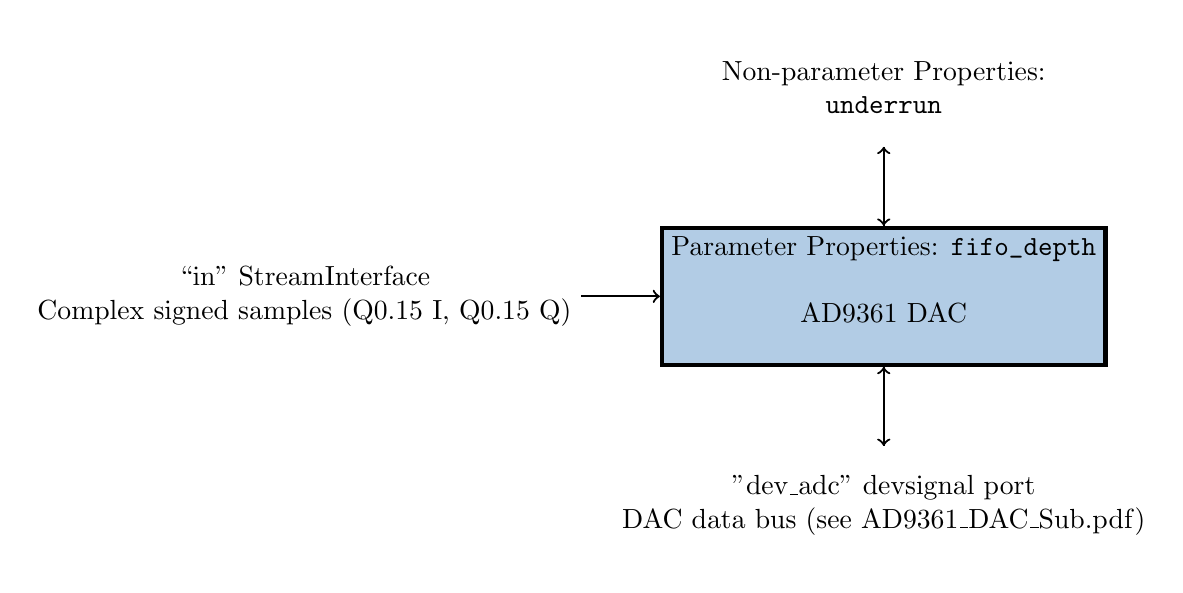
\begin{tikzpicture}[% List of styles applied to all, to override specify on a case-by-case
			every node/.style={
				align=center,  		% use this so that the "\\" for line break works
				minimum size=1.5cm	% creates space above and below text in rectangle
			},
			every edge/.style={draw,thick}
		]
		\node[rectangle,ultra thick,draw=black,fill=blue,minimum width=5 cm](R2){Parameter Properties: \verb+fifo_depth+ \\ \\ \Comp \\};
		\node[rectangle,draw=white,fill=white](R3)[below= of R2]{"dev\_adc" devsignal port\\ DAC data bus (see AD9361\_DAC\_Sub.pdf)};
		\node[rectangle,draw=white,fill=white](R4)[left= of R2]{``in" StreamInterface \\ Complex signed samples (Q0.15 I, Q0.15 Q)};
		\node[rectangle,draw=white,fill=white](R5)[above= of R2]{Non-parameter Properties:\\\verb+underrun+};
		\path[->]
		(R3)edge []	node [] {} (R2)
		(R2)edge []	node [] {} (R3)
		(R4)edge []	node [] {} (R2)
		(R2)edge []	node [] {} (R5)
		(R5)edge []	node [] {} (R2)
		;
	\end{tikzpicture}
\end{center}

\section*{Source Dependencies}
\subsection*{\comp.hdl}
\begin{itemize}
	\item opencpi/hdl/devices/ad9361\_dac.hdl/ad9361\_dac.vhd
	\item opencpi/hdl/primitives/util/dac\_fifo.vhd
	\item opencpi/hdl/primitives/util/util\_pkg.vhd
	\item opencpi/hdl/primitives/util/sync\_status.vhd
	\item opencpi/hdl/primitives/bsv/imports/SyncFIFO.v
	\item opencpi/hdl/primitives/bsv/imports/SyncResetA.v
	\item opencpi/hdl/primitives/bsv/imports/SyncHandshake.v
	\item opencpi/hdl/primitives/bsv/bsv\_pkg.vhd
\end{itemize}
\begin{landscape}

	\section*{Component Spec Properties}
	\begin{scriptsize}
		\begin{tabular}{|p{3.75cm}|p{1.25cm}|p{2cm}|p{2.75cm}|p{1.5cm}|p{1.5cm}|p{1cm}|p{6.62cm}|}
			\hline
			\rowcolor{blue}
			Name               & Type & SequenceLength & ArrayDimensions & Accessibility      & Valid Range & Default & Usage                                                                               \\
			\hline
			\verb+underrun+    & Bool & -              & -               & Volatile, Writable    & Standard    & -       & Flag set when DAC tries to send a sample and the DAC FIFO is empty. Once high, this flag is not cleared (i.e. set low) until the property is written to again (the flag clears regardless of write value, i.e. writing true or false both result in a value of false).\\
			\hline
		\end{tabular}
	\end{scriptsize}

	\section*{Worker Properties}
	\subsection*{\comp.hdl}
	\begin{scriptsize}
		\begin{tabular}{|p{2cm}|p{2cm}|p{1cm}|p{2cm}|p{2cm}|p{2cm}|p{2cm}|p{1cm}|p{5.95cm}|}
			\hline
			\rowcolor{blue}
			Scope        & Name                 & Type & SequenceLength & ArrayDimensions & Accessibility & Valid Range        & Default & Usage                                                                                                                  \\
			\hline
			Property     & \verb+fifo_depth+    & ULong& -              & -               & Parameter     & Standard           & 64      & Depth in number of samples of the control-to-DAC clock domain crossing FIFO. \\
			\hline
		\end{tabular}
	\end{scriptsize}

	\section*{Component Ports}
	\begin{scriptsize}
		\begin{tabular}{|p{2cm}|p{1.5cm}|p{4cm}|p{1.5cm}|p{1.5cm}|p{10.75cm}|}
			\hline
			\rowcolor{blue}
			Name & Producer & Protocol           & Optional & Advanced & Usage                  \\
			\hline
			in   & False    & iqstream\_protocol & False     & -        & Complex signed samples (Q0.15 I, Q0.15 Q). \\
			\hline
		\end{tabular}
	\end{scriptsize}

	\section*{Worker Interfaces}
	\subsection*{\comp.hdl}
	\begin{scriptsize}
		\begin{tabular}{|p{2cm}|p{1.5cm}|p{1.5cm}|p{1.5cm}|p{15.18cm}|}
			\hline
			\rowcolor{blue}
			Type            & Name & DataWidth & Advanced & Usage                  \\
			\hline
			StreamInterface & in   & 32        & -        & Complex signed samples (Q0.15 I, Q0.15 Q). This port ingests data and forces backpressure. Because both a "pulling" pressure from the DAC clock and potentially limited "pushing pressure" from this port exists, it is possible for a value to be clocked to the DAC while no new value was yet seen at the in port. This event is monitored via the \verb+underrun+ property.  \\
			\hline
		\end{tabular}
	\end{scriptsize} \\ \\
	\begin{scriptsize}
		\begin{tabular}{|p{1.75cm}|p{2.25cm}|p{1.25cm}|p{1.25cm}|p{1.25cm}|p{3cm}|p{1.4cm}|p{0.9cm}|p{6.88cm}|}
			\hline
			\rowcolor{blue}
			Type                       & Name                            & Count & Optional & Master                & Signal                & Direction                  & Width                    & Description                                                                                                                  \\
			\hline
			\multirow{15}{*}{\DevSignal{}} & \multirow{15}{*}{dev\_dac} & \multirow{15}{*}{1} & \multirow{15}{*}{False} & \multirow{15}{*}{True}  & present & Output&1& Value is hardcoded to logic 1 inside this worker. \\
			\cline{6-9}
			&             &        &     &      & dac\_clk     & Input     & 1      & Clock for dac\_ready, dac\_take, dac\_data\_I, and dac\_data\_Q. \\
			\cline{6-9}
			&             &        &     &      & dac\_ready   & Output    & 1      & Indicates that the dac\_data\_I and dac\_data\_Q are valid/ready to be latched on the next rising edge of adc\_clk. \\
			\cline{6-9}
			&             &        &     &      & dac\_take    & Input     & 1      & Indicates that dac\_data\_I and dac\_data\_Q were latched on the previous rising edge of dac\_clk. If in the previous clock cycle dac\_ready was 1, the values of dac\_data\_I and dac\_data\_Q should not be allowed to update with a new sample until dac\_take is 1. \\
			\cline{6-9}
			&             &        &     &      & dac\_data\_I & Output    & 12     & Signed Q0.11 I value of DAC sample corresponding to RX channel 1. \\
			\cline{6-9}
			&             &        &     &      & dac\_data\_Q & Output    & 12     & Signed Q0.11 Q value of DAC sample corresponding to RX channel 1. \\
			\hline
		\end{tabular}
	\end{scriptsize}
\end{landscape}

\section*{Control Timing and Signals}
\subsection*{Clock Domains}
The \Comp{}.hdl device worker contains two clock domains: the clock from the control plane, and the dac\_clk clock from the \devsignal{}. It is expected that the control plane clock is faster than the dac\_clk clock in order to prevent a FIFO underrun (monitored via the \verb+underrun+ property). Note that the clock rate of dac\_clk is equivalent to half the clock rate of the AD9361 DATA\_CLK\_P pin\cite{dac_sub_comp_datasheet} and that the AD9361 DATA\_CLK\_P rate's range is 2,083,333 Hz to 61,440,000 Hz. As such, always running this worker with a minimum control plane clock rate of 30,720,000 Hz will prevent underrun under all circumstances.
\subsection*{Latency}
The latency from the input port to the \devsignal{} data bus is both both non-deterministic and dynamic. Non-determinism exists as a result of the data flowing through an asynchronous FIFO with each side in a different clock domain. Runtime dynamism exists as a result of the AD9361 DATA\_CLK\_P clock, and therefore the dac\_clk clock rates, being runtime dynamic. The use of any FIFO, synchronous or asynchronous, between the input port and the \devsignal{} also creates runtime dynamism in latency.
\subsection*{Backpressure}
Backpressure is transferred from the \devsignal{}'s dac\_clk clock to the input port. The input port is expected to frequently experience backpressure in order to prevent a FIFO underrun.

\section*{Performance and Resource Utilization}
\subsubsection*{\comp.hdl}
Fmax refers to the maximum allowable clock rate for any registered signal paths within a given clock domain for an FPGA design. Fmax in the table below is specific only to this worker and represents the maximum possible Fmax for any OpenCPI bitstream built with this worker included. Note that the Fmax value for a given clock domain for the final bitstream is often worse than the Fmax specific to this worker, even if this worker is the only one included in the bitstream. Note also that the dev\_dac's dac\_clk clock rate will only ever go as high as half of the AD9361's DATA\_CLK\_P rate, or half of 245.76 MHz\cite{adi_ug570} which is 122.88 MHz. \\ \\
Table entries are a result of building the woker with the following parameter property sets:
\begin{itemize}
	\item \verb+fifo_depth+=64
\end{itemize}
% see performance_and_resource_utilization.txt
\begin{scriptsize}
	\begin{tabular}{|M{4.2cm}|M{1.1cm}|M{1.1cm}|M{2.3cm}|M{2.7cm}|M{1.9cm}|M{1.3cm}|}
		\hline
    \rowcolor{blue}
    Device                                 & Registers (typical) & LUTS (typical) & \multicolumn{2}{c|}{Fmax (typical)}  & Memory/Special Functions & Design Suite \\
		\hline
    \rowcolor{blue}
		                                       &           &      & control plane clock & dev\_dac.dac\_clk clock &           &          \\
		\hline
		\multirow{2}{*}{Zynq XC7Z020-1-CLG484} & 149       & 126  & 245 MHz \textsuperscript{\ref{abc}} & 233 MHz \textsuperscript{\ref{abc}} & 1 RAMB18 & Vivado 2017.1 \\
		\cline{2-7}
		                                       & 169       & 297  & 410 MHz             & 419 MHz                 & 8 RAM64M  & ISE 14.7 \\
		\hline
		Virtex-6 XC6VLX240T-1-FF1156           & 169       & 289  & 388 MHz             & 391 MHz                 & 8 RAM64M  & ISE 14.7 \\
		\hline
		Stratix IV EP4SGX230K-C2-F40           & 148       & 166  & \ref{quartustiming} & \ref{quartustiming} & 1,536 block memory bits & Quartus Prime 15.1 \\
		\hline
	\end{tabular}
\end{scriptsize} \\ \\
\footnotetext[1]{\label{abc}These measurements were the result of a Vivado timing analysis which was different from the Vivado analysis performed by default for OpenCPI worker builds. For more info see Appendix \ref{appendix}}
\footnotetext[2]{\label{quartustiming}Quartus does not perform timing analysis at the OpenCPI worker build (i.e. synthesis) stage.}
\pagebreak
\section*{Test and Verification}
\subsection*{Theory of Operation}
The AD9361 has a Built In Self Test (BIST) mode cable of validating in-situ the digital RX/TX data paths without the need for additional external equipment. One of the BIST configurations enables a Linear Feedback Shift Register (LFSR) within the AD9361 and sends the LFSR output to AD9361's ADC data pins. The LFSR generates a Pseudo Random Bit Sequence (PRBS). By using the LFSR algorithm to verify data fidelity after the RX data is registered inside the FPGA, the AD9361-to-FPGA digital RX data path is verified. An additional BIST configuration exists which performs a digital TX-to-RX loopback on the AD9361. By first validating the RX data path with the PRBS BIST, then running a loopback BIST while sending generating LFSR data to the AD9361 TX path while using the LFSR algorithm to verify data fidently after the RX data is registered inside the FPGA, the entire FPGA-to-AD9361-to-FPGA digital RX/TX data path is verfied. For more information on the BIST modes see \cite{adi_bist_doc} and \cite{adi_ug570}. \\ \\
The \comp{}.hdl unit test performs an in-situ hardware test on either a Zedboard / FMCOMMS2/3 or x86 / ML605 / FMCOMMS2/3 hardware platform. The unit test currently only tests the AD9361 in its single channel LVDS mode. Note that AD9361 also supports two-channel mode and 4 non-LVDS (CMOS) modes. The unit test validates not only the \comp{}.hdl device worker, but the entire command/control and RX/TX data paths both in software and hardware. \\ \\
The unit test first runs multiple ocpirun applications which use the AD9361 BIST PRBS mode and save the first 8192 samples output from the ad9361\_adc.hdl output port to a binary file. A Bit Error Rate (BER) is then calculated on each output file and verified to be 0\%. These data fidelty tests are run across the full range of possible AD9361 sample rates, (2.083334 Msps complex - 61.44 Msps complex for a single channel is the full range when the AD9361 FIR filter is disabled, note that said filter is disabled for all tests). The ad9361\_adc.hdl's \verb+overrun+ property is verified to be false for apps running as long as 10 seconds at the max sample rate. All of these tests are run for both 1R1T timing and 2R2T AD9361 timing modes. For more information on these AD9361 modes, see \cite{adi_ug570}. \\ \\
The unit test next runs multiple ocpirun applications which use the AD9361 BIST loopback mode and save the first 8192 samples output from the ad9361\_adc.hdl output port to a binary file. The applications utilize an HDL worker which generates LFSR data (similar to the LFSR data generated on the AD9361 for the PRBS BIST) and sends this data out the TX path\footnote{For more information, see Data Src Component Data Sheet}. A Bit Error Rate (BER) is then calculated on each output file and verified to be 0\%. These data fidelty tests are run across the full range of possible AD9361 sample rates, (2.083334 Msps complex - 61.44 Msps complex for a single channel is the full range when the AD9361 FIR filter is disabled, note that said filter is disabled for all tests). The \verb+underrun+ property is verified to be false for apps running as long as 10 seconds at the max sample rate. All of these tests are run for both 1R1T timing and 2R2T AD9361 timing modes. For more information on these AD9361 modes, see \cite{adi_ug570}.
\subsection*{Hardware Configuration}
The \comp{}.hdl unit test requires an FMCOMMS2 or FMCOMMS3 card (which has an AD9361 on board) and an ML605 or Zedboard. On ML605, the FMCOMMS3 must be in the FMC LPC slot due to known TX data fidelity issues with the FMC HPC slot.
\subsection*{Build Instructions}
The \comp{}.test directory contains the \comp{}.hdl unit test. The test can be built on a development machine from within this directory by running the following command to build for ML605 deployment:
\lstset{language=bash, columns=flexible, breaklines=true, prebreak=\textbackslash, basicstyle=\ttfamily, showstringspaces=false,upquote=true, aboveskip=\baselineskip, belowskip=\baselineskip}
\begin{lstlisting}
ocpidev build --hdl-platform ml605
\end{lstlisting}
The following command builds for Zedboard deployment:
\begin{lstlisting}
OCPI_TARGET_PLATFORM=xilinx13_3 ocpidev build --hdl-platform zed
\end{lstlisting}
\subsection*{Execution Instructions}
When executing on an x86/ML605 machine, the \texttt{LD\_LIBRARY\_PATH} environment variable must be prepended with the location of the libusb install directory which was determined when performing the AngryViper Xilinx ISE installation instructions\cite{vendor_tools_install} (most likely location is /usr/local/lib/). If it does not matter which ML605 FMC slot is tested, the ML605 test should be executed by running the following command. Using this command, it is possible for either ML605 FMC slot to be used for AD9361 tests at runtime.
\begin{lstlisting}
LD_LIBRARY_PATH=<libusb-install-location>:$LD_LIBRARY_PATH make tests
\end{lstlisting}
To test the ML605 for a specific FMCOMMS2/3 FMC slot location, the \texttt{OCPI\_LIBRARY\_PATH} environment variable must be prepended with the location of the FPGA bitstream for the desired FMC LPC/HPC slot. The command is as follows:
\begin{lstlisting}
LD_LIBRARY_PATH=<libusb-install-location>:$LD_LIBRARY_PATH OCPI_LIBRARY_PATH=<path-to-bitstream>:$OCPI_LIBRARY_PATH make tests
\end{lstlisting}
To run on the Zedboard, the built \comp{}.test directory must either be mounted from the development machine to the Zedboard, or copied to the Zedboard. From within the \comp{}.test directory, the follow command executes the test natively on the Zedboard:
\begin{lstlisting}
./ad9361_dac_test_app
\end{lstlisting}
Upon completion of a successful test, PASSED is printed to the screen and a value of 0 is returned. Upon failure, FAILED is printed to the screen and a non-zero value is returned.
\subsection*{Troubleshooting}
This unit test is in need of more robust error messaging. If a failure occurs but the test completed, the screen will output a diff between a generated log file odata/AD9361\_BIST\_PRBS.log and a golden log file. If a failure occurs before the test was completed, there is sometimes not a good error message generated. Upon failure, the logs should be checked to ensure the error was not one which prevented the test from being run. Log files are also saved which capture the stdout/stderr for each of the multiple ocpirun calls, e.g. odata/app\_2.083334e6sps\_fir0\_0\_1sec\_prbs.log.

\pagebreak
\begin{thebibliography}{1}

\bibitem{ad9361} AD9361 Datasheet and Product Info \\
\url{http://www.analog.com/en/products/rf-microwave/integrated-transceivers-transmitters-receivers/wideband-transceivers-ic/ad9361.html}
\bibitem{adi_ug570} AD9361 Reference Manual UG-570\\
AD9361\_Reference\_Manual\_UG-570.pdf
\bibitem{adi_bist_doc} AD9361 BIST FAQ \\
\url{https://ez.analog.com/servlet/JiveServlet/download/11828-2-28791/AD9361%20BIST%20FAQ.pdf}
\bibitem{vendor_tools_install} FPGA Vendor Tools Installation Guide \\
FPGA\_Vendor\_Tools\_Installation\_Guide.pdf
\bibitem{dac_sub_comp_datasheet} AD361 DAC Sub Component Data Sheet \\AD9361\_DAC\_Sub.pdf

\end{thebibliography}
\pagebreak
\section{Appendix - Vivado Timing Analysis} \label{appendix}

The Vivado timing report that OpenCPI runs for device workers may erroneously report a max delay for a clocking path which should have been ignored. Custom Vivado tcl commands had to be run for this device worker to extract pertinent information from Vivado timing analysis. After building the worker, the following commands were run from the base project directory (after the Vivado settings64.sh was sourced):
\begin{lstlisting}
cd hdl/devices/
vivado -mode tcl
\end{lstlisting}
Then the following commands were run inside the Vivado tcl terminal:
\begin{lstlisting}
open_project ad9361_dac.hdl/target-zynq/ad9361_dac_rv.xpr
synth_design -part xc7z020clg484-1 -top ad9361_dac_rv -mode out_of_context
create_clock -name clk1 -period 0.001 [get_nets {ctl_in[Clk]}]
create_clock -name clk2 -period 0.001 [get_nets {dev_dac_in[dac_clk]}]
set_clock_groups -asynchronous -group [get_clocks clk1] -group [get_clocks clk2]
report_timing -delay_type min_max -sort_by slack -input_pins -group clk1
report_timing -delay_type min_max -sort_by slack -input_pins -group clk2
\end{lstlisting}
The following is the output of the timing reports. The Fmax for the control plane clock for this worker is computed as the maximum magnitude slack with a control plane clock of 1 ps plus 2 times the assumed 1 ps control plane clock period (4.075 ns + 0.002 ns = 4.077 ns, 1/4.077 ns = 245.28 MHz). The Fmax for the dac\_clk clock from the devsignal is computed as the maximum magnitude slack with dac\_clk of 1 ps plus 2 times the assumed 1 ps dac\_clk period (4.285 ns + 0.002 ns = 4.287 ns, 1/4.287 ns = 233.26 MHz).
\fontsize{6}{12}\selectfont
\begin{lstlisting}
Vivado% report_timing -delay_type min_max -sort_by slack -input_pins -group clk1

Timing Report

Slack (VIOLATED) :        -4.075ns  (required time - arrival time)
  Source:                 IN_port/fifo/data0_reg_reg[12]/C
                            (rising edge-triggered cell FDRE clocked by clk1  {rise@0.000ns fall@0.001ns period=0.001ns})
  Destination:            worker/fifo/fifo/fifoMem_reg/DIADI[9]
                            (rising edge-triggered cell RAMB18E1 clocked by clk1  {rise@0.000ns fall@0.001ns period=0.001ns})
  Path Group:             clk1
  Path Type:              Setup (Max at Slow Process Corner)
  Requirement:            0.002ns  (clk1 rise@0.002ns - clk1 rise@0.000ns)
  Data Path Delay:        3.077ns  (logic 1.780ns (57.854%)  route 1.297ns (42.146%))
  Logic Levels:           4  (CARRY4=3 LUT2=1)
  Clock Path Skew:        -0.049ns (DCD - SCD + CPR)
    Destination Clock Delay (DCD):    0.924ns = ( 0.926 - 0.002 ) 
    Source Clock Delay      (SCD):    0.973ns
    Clock Pessimism Removal (CPR):    0.000ns
  Clock Uncertainty:      0.035ns  ((TSJ^2 + TIJ^2)^1/2 + DJ) / 2 + PE
    Total System Jitter     (TSJ):    0.071ns
    Total Input Jitter      (TIJ):    0.000ns
    Discrete Jitter          (DJ):    0.000ns
    Phase Error              (PE):    0.000ns

    Location             Delay type                Incr(ns)  Path(ns)    Netlist Resource(s)
  -------------------------------------------------------------------    -------------------
                         (clock clk1 rise edge)       0.000     0.000 r  
                                                      0.000     0.000 r  ctl_in[Clk] (IN)
                         net (fo=114, unset)          0.973     0.973    IN_port/fifo/ctl_in[Clk]
                         FDRE                                         r  IN_port/fifo/data0_reg_reg[12]/C
  -------------------------------------------------------------------    -------------------
                         FDRE (Prop_fdre_C_Q)         0.518     1.491 r  IN_port/fifo/data0_reg_reg[12]/Q
                         net (fo=3, unplaced)         0.488     1.979    IN_port/fifo/IN_data[4]
                                                                      r  IN_port/fifo/fifoMem_reg_i_24/I0
                         LUT2 (Prop_lut2_I0_O)        0.295     2.274 r  IN_port/fifo/fifoMem_reg_i_24/O
                         net (fo=1, unplaced)         0.000     2.274    IN_port/fifo/fifoMem_reg_i_24_n_0
                                                                      r  IN_port/fifo/fifoMem_reg_i_5/S[0]
                         CARRY4 (Prop_carry4_S[0]_CO[3])
                                                      0.513     2.787 r  IN_port/fifo/fifoMem_reg_i_5/CO[3]
                         net (fo=1, unplaced)         0.009     2.796    IN_port/fifo/fifoMem_reg_i_5_n_0
                                                                      r  IN_port/fifo/fifoMem_reg_i_4/CI
                         CARRY4 (Prop_carry4_CI_CO[3])
                                                      0.117     2.913 r  IN_port/fifo/fifoMem_reg_i_4/CO[3]
                         net (fo=1, unplaced)         0.000     2.913    IN_port/fifo/fifoMem_reg_i_4_n_0
                                                                      r  IN_port/fifo/fifoMem_reg_i_3/CI
                         CARRY4 (Prop_carry4_CI_O[1])
                                                      0.337     3.250 r  IN_port/fifo/fifoMem_reg_i_3/O[1]
                         net (fo=1, unplaced)         0.800     4.050    worker/fifo/fifo/sD_IN[9]
                         RAMB18E1                                     r  worker/fifo/fifo/fifoMem_reg/DIADI[9]
  -------------------------------------------------------------------    -------------------

                         (clock clk1 rise edge)       0.002     0.002 r  
                                                      0.000     0.002 r  ctl_in[Clk] (IN)
                         net (fo=114, unset)          0.924     0.926    worker/fifo/fifo/ctl_in[Clk]
                         RAMB18E1                                     r  worker/fifo/fifo/fifoMem_reg/CLKBWRCLK
                         clock pessimism              0.000     0.926    
                         clock uncertainty           -0.035     0.891    
                         RAMB18E1 (Setup_ramb18e1_CLKBWRCLK_DIADI[9])
                                                     -0.916    -0.025    worker/fifo/fifo/fifoMem_reg
  -------------------------------------------------------------------
                         required time                         -0.025    
                         arrival time                          -4.050    
  -------------------------------------------------------------------
                         slack                                 -4.075    




report_timing: Time (s): cpu = 00:00:08 ; elapsed = 00:00:09 . Memory (MB): peak = 2080.828 ; gain = 485.520 ; free physical = 16892 ; free virtual = 84602
Vivado% report_timing -delay_type min_max -sort_by slack -input_pins -group clk2

Timing Report

Slack (VIOLATED) :        -4.285ns  (required time - arrival time)
  Source:                 worker/fifo/fifo/dGDeqPtr_reg[1]/C
                            (rising edge-triggered cell FDCE clocked by clk2  {rise@0.000ns fall@0.001ns period=0.001ns})
  Destination:            worker/fifo/fifo/fifoMem_reg/ENARDEN
                            (rising edge-triggered cell RAMB18E1 clocked by clk2  {rise@0.000ns fall@0.001ns period=0.001ns})
  Path Group:             clk2
  Path Type:              Setup (Max at Slow Process Corner)
  Requirement:            0.002ns  (clk2 rise@0.002ns - clk2 rise@0.000ns)
  Data Path Delay:        3.760ns  (logic 1.061ns (28.220%)  route 2.699ns (71.780%))
  Logic Levels:           3  (LUT4=2 LUT6=1)
  Clock Path Skew:        -0.049ns (DCD - SCD + CPR)
    Destination Clock Delay (DCD):    0.924ns = ( 0.926 - 0.002 ) 
    Source Clock Delay      (SCD):    0.973ns
    Clock Pessimism Removal (CPR):    0.000ns
  Clock Uncertainty:      0.035ns  ((TSJ^2 + TIJ^2)^1/2 + DJ) / 2 + PE
    Total System Jitter     (TSJ):    0.071ns
    Total Input Jitter      (TIJ):    0.000ns
    Discrete Jitter          (DJ):    0.000ns
    Phase Error              (PE):    0.000ns

    Location             Delay type                Incr(ns)  Path(ns)    Netlist Resource(s)
  -------------------------------------------------------------------    -------------------
                         (clock clk2 rise edge)       0.000     0.000 r  
                                                      0.000     0.000 r  dev_dac_in[dac_clk] (IN)
                         net (fo=35, unset)           0.973     0.973    worker/fifo/fifo/dev_dac_in[dac_clk]
                         FDCE                                         r  worker/fifo/fifo/dGDeqPtr_reg[1]/C
  -------------------------------------------------------------------    -------------------
                         FDCE (Prop_fdce_C_Q)         0.518     1.491 r  worker/fifo/fifo/dGDeqPtr_reg[1]/Q
                         net (fo=3, unplaced)         0.983     2.474    worker/fifo/fifo/p_0_in[0]
                                                                      r  worker/fifo/fifo/dNotEmptyReg_i_5/I0
                         LUT6 (Prop_lut6_I0_O)        0.295     2.769 r  worker/fifo/fifo/dNotEmptyReg_i_5/O
                         net (fo=1, unplaced)         0.449     3.218    worker/fifo/fifo/dNotEmptyReg_i_5_n_0
                                                                      r  worker/fifo/fifo/dNotEmptyReg_i_3/I3
                         LUT4 (Prop_lut4_I3_O)        0.124     3.342 r  worker/fifo/fifo/dNotEmptyReg_i_3/O
                         net (fo=3, unplaced)         0.467     3.809    worker/fifo/fifo/dNextNotEmpty__12
                                                                      r  worker/fifo/fifo/fifoMem_reg_i_1/I0
                         LUT4 (Prop_lut4_I0_O)        0.124     3.933 r  worker/fifo/fifo/fifoMem_reg_i_1/O
                         net (fo=1, unplaced)         0.800     4.733    worker/fifo/fifo/fifoMem_reg_i_1_n_0
                         RAMB18E1                                     r  worker/fifo/fifo/fifoMem_reg/ENARDEN
  -------------------------------------------------------------------    -------------------

                         (clock clk2 rise edge)       0.002     0.002 r  
                                                      0.000     0.002 r  dev_dac_in[dac_clk] (IN)
                         net (fo=35, unset)           0.924     0.926    worker/fifo/fifo/dev_dac_in[dac_clk]
                         RAMB18E1                                     r  worker/fifo/fifo/fifoMem_reg/CLKARDCLK
                         clock pessimism              0.000     0.926    
                         clock uncertainty           -0.035     0.891    
                         RAMB18E1 (Setup_ramb18e1_CLKARDCLK_ENARDEN)
                                                     -0.443     0.448    worker/fifo/fifo/fifoMem_reg
  -------------------------------------------------------------------
                         required time                          0.448    
                         arrival time                          -4.733    
  -------------------------------------------------------------------
                         slack                                 -4.285    




\end{lstlisting}

\end{document}

